\documentclass{article}

\usepackage[letterpaper]{geometry}
\usepackage{tgpagella}
\usepackage{amsmath}
\usepackage{amssymb}
\usepackage{amsthm}
\usepackage{tikz}
\usepackage{minted}
\usepackage{physics}
\usepackage{siunitx}
\usepackage{mhchem}
\usepackage{float}
\usepackage{endiagram}
\usepackage{gnuplot-lua-tikz}

\sisetup{detect-all}
\newtheorem{plm}{Problem}
\renewcommand*{\proofname}{Solution}

\title{4271 HW 4}
\author{Duncan Wilkie}
\date{8 March 2023}

\begin{document}

\maketitle

\begin{plm}
  For the following gamma transitions, give all permitted multipoles and indicate which might be the most intense:
  \begin{enumerate}
  \item $\frac{9}{2}^{-} \mapsto \frac{7}{2}^{+}$
  \item $\frac{1}{2}^{-} \mapsto \frac{7}{2}^{-}$
  \item ${1}^{-} \mapsto 2^{+}$
  \item $4^{+} \mapsto 2^{+}$
  \item $3^{+} \mapsto 3^{+}$
  \end{enumerate}
\end{plm}

\begin{proof}
  In the first case, the vector diference yields possible $L$ of $1, 2, 3, 4, 5, 6, 7$.
  The parity is $(-1)^{L}$ for an electric transition, and $-(-1)^{L}$ for a magnetic transition,
  so these correspond to an electric dipole, magnetic quadrupole, electric octupole, magnetic 16-pole, etc. on up to electric 128-pole.
  In general, the lower-$L$ transitions tend to be more intense.

  Proceeding similarly, but in less detail for the other cases, with the most intese guess underlined,
  \[
    3 \leq J_{f}- J_{i} \leq 4 \Leftrightarrow L = 3, 4 \Rightarrow \textrm{\underline{magnetic octupole} and electric 16-pole transitions.}
  \]
  \[
    1 \leq J_{f} - J_{i} \leq 3 \Rightarrow L = 1, 2, 3 \Rightarrow \textrm{\underline{electric dipole}, magnetic quadrupole,
      and electric octupole transitions.}
  \]
  \[
    2 \leq J_{f} - J_{i} \leq 6 \Rightarrow L = 2, 3, 4, 5, 6 \Rightarrow \textrm{electric \underline{quadrupole}, magnetic octupole,
      electic 16-pole,}\]
  \[
    \text{magnetic 32-pole, and electric 64-pole transitions.}
  \]

  In the last case, there can be no gamma transition, as there is no change in angular momentum.
\end{proof}

\begin{plm}
  An even-$Z$, even-$N$ nucleus has the following sequence of levels: $0+$ (ground state), $2+$ (\SI{89}{keV}), $4+$ (\SI{288}{keV}),
  $6+$ (\SI{585}{keV}), $0+$ (\SI{1050}{keV}), $2+$ (\SI{1129}{keV}).
  Drawn an energy level diagram and show all reasonbably probable gamma-ray transitions and their dominant multipole assignments.
\end{plm}

\begin{proof}
  Possible transitions:
  \begin{center}
    \begin{endiagram}
      \ENcurve{11, 10, 10}
      \node[above] at (N1-1) {$2^{+}$};
      \node[below,xshift=0.6cm] at (N1-2) {$0^{+}$};
      \ShowGain[label=Electric quadrupole]
      \ShowNiveaus[niveau=N1-1]
      \ENcurve{5, 2, 1, 0}
      \ShowEa[max=all]
      \node[above] at (N2-1) {$6^{+}$};
      \ShowEa[from = {(N2-1) to (N2-2)}, label=Electric 16-pole]
      \node[below] at (N2-2) {$4^{+}$};
      \node[below] at (N2-3) {$2^{+}$};
      \ShowEa[from = {(N2-2) to (N2-3)}, label=Electric quadrupole]
      \node[below] at (N2-4) {$0^{+}$};
      \ShowEa[from = {(N2-3) to (N2-4)}, label=Electric quadrupole]
      \ShowNiveaus
    \end{endiagram}
  \end{center}
  There is also an electric quadrupole transition from the highest $2^{+}$ state to the lowest $0^{+}$;
  the chemistry package I yoinked this drawing code from doesn't support that kind of a thing so easily.
\end{proof}

\begin{plm}
  The excited states of $\ce{^{174}Hf}$ have two similar rotational bands, with energies (in \si{MeV}) given in the following table.
  Calculate the moments of inertia for these two bands and comment on the difference.
  \begin{table}[H]
    \centering
    \begin{tabular}{|c|c|c|c|c|c|c|c|}
      \hline
      & $E(0^{+})$ & $E(2^{+})$ & $E(4^{+})$ & $E(6^{+})$ & $E(8^{+})$ & $E(10^{+})$ & $E(12^{+})$ \\
      \hline
      Band 1 & 0 & 0.091 & 0.297 & 0.608 & 1.010 & 1.486 & 2.021 \\
      \hline
      Band 2 & 0.827 & 0.900 & 1.063 & 1.307 & 1.630 & 2.026 & 2.489 \\
      \hline
    \end{tabular}
  \end{table}
\end{plm}

\begin{proof}
  A quick linear fit yields:
  \begin{center}
    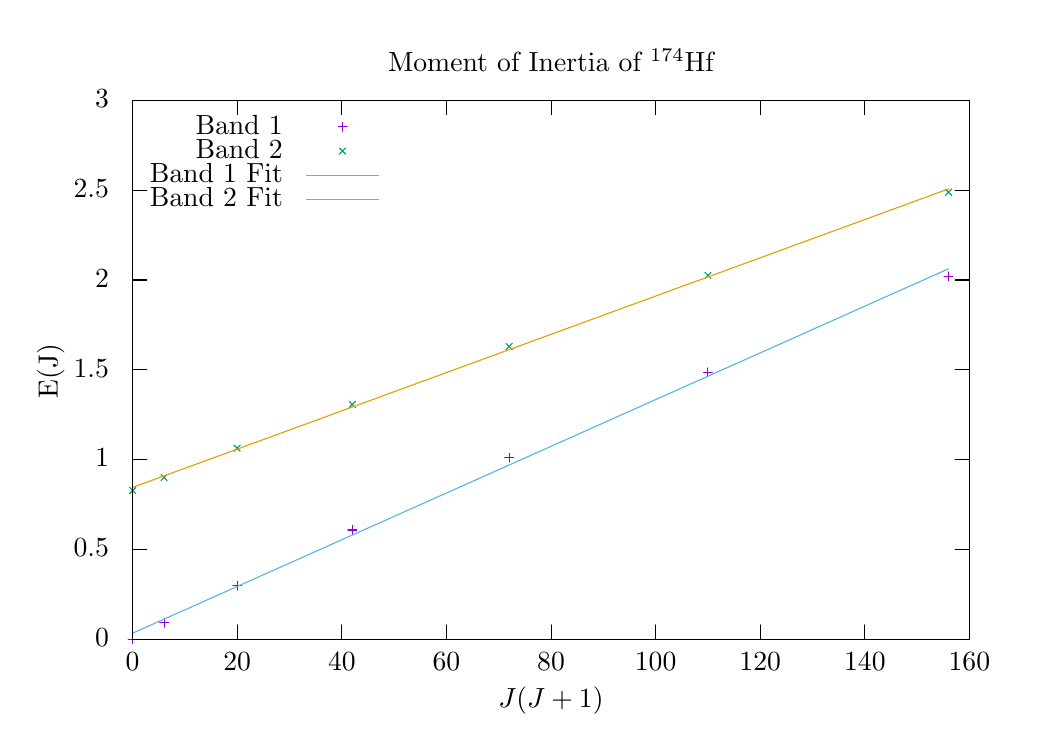
\begin{tikzpicture}[gnuplot]
%% generated with GNUPLOT 5.4p4 (Lua 5.3; terminal rev. Jun 2020, script rev. 115)
%% Thu 09 Mar 2023 08:24:07 PM CST
\path (0.000,0.000) rectangle (12.500,8.750);
\gpcolor{color=gp lt color border}
\gpsetlinetype{gp lt border}
\gpsetdashtype{gp dt solid}
\gpsetlinewidth{1.00}
\draw[gp path] (1.320,0.985)--(1.500,0.985);
\draw[gp path] (11.947,0.985)--(11.767,0.985);
\node[gp node right] at (1.136,0.985) {$0$};
\draw[gp path] (1.320,2.125)--(1.500,2.125);
\draw[gp path] (11.947,2.125)--(11.767,2.125);
\node[gp node right] at (1.136,2.125) {$0.5$};
\draw[gp path] (1.320,3.265)--(1.500,3.265);
\draw[gp path] (11.947,3.265)--(11.767,3.265);
\node[gp node right] at (1.136,3.265) {$1$};
\draw[gp path] (1.320,4.405)--(1.500,4.405);
\draw[gp path] (11.947,4.405)--(11.767,4.405);
\node[gp node right] at (1.136,4.405) {$1.5$};
\draw[gp path] (1.320,5.545)--(1.500,5.545);
\draw[gp path] (11.947,5.545)--(11.767,5.545);
\node[gp node right] at (1.136,5.545) {$2$};
\draw[gp path] (1.320,6.685)--(1.500,6.685);
\draw[gp path] (11.947,6.685)--(11.767,6.685);
\node[gp node right] at (1.136,6.685) {$2.5$};
\draw[gp path] (1.320,7.825)--(1.500,7.825);
\draw[gp path] (11.947,7.825)--(11.767,7.825);
\node[gp node right] at (1.136,7.825) {$3$};
\draw[gp path] (1.320,0.985)--(1.320,1.165);
\draw[gp path] (1.320,7.825)--(1.320,7.645);
\node[gp node center] at (1.320,0.677) {$0$};
\draw[gp path] (2.648,0.985)--(2.648,1.165);
\draw[gp path] (2.648,7.825)--(2.648,7.645);
\node[gp node center] at (2.648,0.677) {$20$};
\draw[gp path] (3.977,0.985)--(3.977,1.165);
\draw[gp path] (3.977,7.825)--(3.977,7.645);
\node[gp node center] at (3.977,0.677) {$40$};
\draw[gp path] (5.305,0.985)--(5.305,1.165);
\draw[gp path] (5.305,7.825)--(5.305,7.645);
\node[gp node center] at (5.305,0.677) {$60$};
\draw[gp path] (6.634,0.985)--(6.634,1.165);
\draw[gp path] (6.634,7.825)--(6.634,7.645);
\node[gp node center] at (6.634,0.677) {$80$};
\draw[gp path] (7.962,0.985)--(7.962,1.165);
\draw[gp path] (7.962,7.825)--(7.962,7.645);
\node[gp node center] at (7.962,0.677) {$100$};
\draw[gp path] (9.290,0.985)--(9.290,1.165);
\draw[gp path] (9.290,7.825)--(9.290,7.645);
\node[gp node center] at (9.290,0.677) {$120$};
\draw[gp path] (10.619,0.985)--(10.619,1.165);
\draw[gp path] (10.619,7.825)--(10.619,7.645);
\node[gp node center] at (10.619,0.677) {$140$};
\draw[gp path] (11.947,0.985)--(11.947,1.165);
\draw[gp path] (11.947,7.825)--(11.947,7.645);
\node[gp node center] at (11.947,0.677) {$160$};
\draw[gp path] (1.320,7.825)--(1.320,0.985)--(11.947,0.985)--(11.947,7.825)--cycle;
\node[gp node center,rotate=-270] at (0.292,4.405) {E(J)};
\node[gp node center] at (6.633,0.215) {$J(J+1)$};
\node[gp node right] at (3.344,7.491) {Band 1};
\gpcolor{rgb color={0.580,0.000,0.827}}
\gpsetpointsize{4.00}
\gp3point{gp mark 1}{}{(1.320,0.985)}
\gp3point{gp mark 1}{}{(1.719,1.192)}
\gp3point{gp mark 1}{}{(2.648,1.662)}
\gp3point{gp mark 1}{}{(4.110,2.371)}
\gp3point{gp mark 1}{}{(6.102,3.288)}
\gp3point{gp mark 1}{}{(8.626,4.373)}
\gp3point{gp mark 1}{}{(11.681,5.593)}
\gp3point{gp mark 1}{}{(3.986,7.491)}
\gpcolor{color=gp lt color border}
\node[gp node right] at (3.344,7.183) {Band 2};
\gpcolor{rgb color={0.000,0.620,0.451}}
\gp3point{gp mark 2}{}{(1.320,2.871)}
\gp3point{gp mark 2}{}{(1.719,3.037)}
\gp3point{gp mark 2}{}{(2.648,3.409)}
\gp3point{gp mark 2}{}{(4.110,3.965)}
\gp3point{gp mark 2}{}{(6.102,4.701)}
\gp3point{gp mark 2}{}{(8.626,5.604)}
\gp3point{gp mark 2}{}{(11.681,6.660)}
\gp3point{gp mark 2}{}{(3.986,7.183)}
\gpcolor{color=gp lt color border}
\node[gp node right] at (3.344,6.875) {Band 1 Fit};
\gpcolor{rgb color={0.337,0.706,0.914}}
\draw[gp path] (3.528,6.875)--(4.444,6.875);
\draw[gp path] (1.320,1.060)--(1.425,1.107)--(1.529,1.154)--(1.634,1.201)--(1.739,1.247)%
  --(1.843,1.294)--(1.948,1.341)--(2.053,1.387)--(2.157,1.434)--(2.262,1.481)--(2.367,1.528)%
  --(2.471,1.574)--(2.576,1.621)--(2.681,1.668)--(2.785,1.715)--(2.890,1.761)--(2.995,1.808)%
  --(3.099,1.855)--(3.204,1.902)--(3.309,1.948)--(3.413,1.995)--(3.518,2.042)--(3.623,2.089)%
  --(3.727,2.135)--(3.832,2.182)--(3.936,2.229)--(4.041,2.276)--(4.146,2.322)--(4.250,2.369)%
  --(4.355,2.416)--(4.460,2.462)--(4.564,2.509)--(4.669,2.556)--(4.774,2.603)--(4.878,2.649)%
  --(4.983,2.696)--(5.088,2.743)--(5.192,2.790)--(5.297,2.836)--(5.402,2.883)--(5.506,2.930)%
  --(5.611,2.977)--(5.716,3.023)--(5.820,3.070)--(5.925,3.117)--(6.030,3.164)--(6.134,3.210)%
  --(6.239,3.257)--(6.344,3.304)--(6.448,3.351)--(6.553,3.397)--(6.658,3.444)--(6.762,3.491)%
  --(6.867,3.537)--(6.972,3.584)--(7.076,3.631)--(7.181,3.678)--(7.286,3.724)--(7.390,3.771)%
  --(7.495,3.818)--(7.600,3.865)--(7.704,3.911)--(7.809,3.958)--(7.914,4.005)--(8.018,4.052)%
  --(8.123,4.098)--(8.228,4.145)--(8.332,4.192)--(8.437,4.239)--(8.542,4.285)--(8.646,4.332)%
  --(8.751,4.379)--(8.856,4.426)--(8.960,4.472)--(9.065,4.519)--(9.169,4.566)--(9.274,4.612)%
  --(9.379,4.659)--(9.483,4.706)--(9.588,4.753)--(9.693,4.799)--(9.797,4.846)--(9.902,4.893)%
  --(10.007,4.940)--(10.111,4.986)--(10.216,5.033)--(10.321,5.080)--(10.425,5.127)--(10.530,5.173)%
  --(10.635,5.220)--(10.739,5.267)--(10.844,5.314)--(10.949,5.360)--(11.053,5.407)--(11.158,5.454)%
  --(11.263,5.500)--(11.367,5.547)--(11.472,5.594)--(11.577,5.641)--(11.681,5.687);
\gpcolor{color=gp lt color border}
\node[gp node right] at (3.344,6.567) {Band 2 Fit};
\gpcolor{rgb color={0.902,0.624,0.000}}
\draw[gp path] (3.528,6.567)--(4.444,6.567);
\draw[gp path] (1.320,2.912)--(1.425,2.950)--(1.529,2.988)--(1.634,3.027)--(1.739,3.065)%
  --(1.843,3.103)--(1.948,3.142)--(2.053,3.180)--(2.157,3.218)--(2.262,3.256)--(2.367,3.295)%
  --(2.471,3.333)--(2.576,3.371)--(2.681,3.409)--(2.785,3.448)--(2.890,3.486)--(2.995,3.524)%
  --(3.099,3.563)--(3.204,3.601)--(3.309,3.639)--(3.413,3.677)--(3.518,3.716)--(3.623,3.754)%
  --(3.727,3.792)--(3.832,3.831)--(3.936,3.869)--(4.041,3.907)--(4.146,3.945)--(4.250,3.984)%
  --(4.355,4.022)--(4.460,4.060)--(4.564,4.099)--(4.669,4.137)--(4.774,4.175)--(4.878,4.213)%
  --(4.983,4.252)--(5.088,4.290)--(5.192,4.328)--(5.297,4.367)--(5.402,4.405)--(5.506,4.443)%
  --(5.611,4.481)--(5.716,4.520)--(5.820,4.558)--(5.925,4.596)--(6.030,4.635)--(6.134,4.673)%
  --(6.239,4.711)--(6.344,4.749)--(6.448,4.788)--(6.553,4.826)--(6.658,4.864)--(6.762,4.903)%
  --(6.867,4.941)--(6.972,4.979)--(7.076,5.017)--(7.181,5.056)--(7.286,5.094)--(7.390,5.132)%
  --(7.495,5.171)--(7.600,5.209)--(7.704,5.247)--(7.809,5.285)--(7.914,5.324)--(8.018,5.362)%
  --(8.123,5.400)--(8.228,5.439)--(8.332,5.477)--(8.437,5.515)--(8.542,5.553)--(8.646,5.592)%
  --(8.751,5.630)--(8.856,5.668)--(8.960,5.707)--(9.065,5.745)--(9.169,5.783)--(9.274,5.821)%
  --(9.379,5.860)--(9.483,5.898)--(9.588,5.936)--(9.693,5.975)--(9.797,6.013)--(9.902,6.051)%
  --(10.007,6.089)--(10.111,6.128)--(10.216,6.166)--(10.321,6.204)--(10.425,6.243)--(10.530,6.281)%
  --(10.635,6.319)--(10.739,6.357)--(10.844,6.396)--(10.949,6.434)--(11.053,6.472)--(11.158,6.511)%
  --(11.263,6.549)--(11.367,6.587)--(11.472,6.625)--(11.577,6.664)--(11.681,6.702);
\gpcolor{color=gp lt color border}
\draw[gp path] (1.320,7.825)--(1.320,0.985)--(11.947,0.985)--(11.947,7.825)--cycle;
\node[gp node center] at (6.633,8.287) {Moment of Inertia of ${^{174}}$Hf};
%% coordinates of the plot area
\gpdefrectangularnode{gp plot 1}{\pgfpoint{1.320cm}{0.985cm}}{\pgfpoint{11.947cm}{7.825cm}}
\end{tikzpicture}

  \end{center}
  The exact fit parameters extracted from gnuplot yield slopes of $0.0130 \pm 0.0002$ and $0.0106 \pm 0.0001$,
  for bands 1 and 2 respectively; the rule for rotational kinetic energy is that
  \[
    E_{rot} = \frac{\hbar^{2}}{2I}[J(J+1)] + E_{k},
  \]
  implying that the moment of inertia in terms of the slope $m$ is, considering $J$ in natural units of $\hbar$,
  \[
    I = \frac{\hbar^{2}}{2m} = \frac{\SI{1}{\hbar^{2}}}{2(\SI{0.013}{})} = \SI{38.5}{}
  \]
  for the first band and
  \[
    I = \frac{\hbar^{2}}{2m} = \frac{\SI{1}{\hbar^{2}}}{2(\SI{0.0106}{})} = \SI{47.2}{}
  \]
  for the second.
\end{proof}

\begin{plm}[Bonus]
  Show explicitly that a uniformly-charged ellipsoid at rest with a total charge of $Ze$ and semi-axes $a$ and $b$ has a quadrupole moment
  \[
    Q = \frac{2}{5}Z\qty(a^{2} - b^{2})
  \]
\end{plm}

\begin{proof}
  First, the volume of an ellipsoid with semi-axes $a$, $b$, $c$: in angular ellipsoidal coordinates,
  in which the angular coordinates from spherical coordinates remain unchanged,
  but the remaining variable parameterizes larger ellipsoidal constant surfaces with semi-axes $a, b, c$,
  \[
    V = \int_{0}^{\pi}\int_{0}^{2\pi}\int_{0}^{1}abcs^{2}\sin\theta dsd\phi d\theta
    = 4\pi abc\qty(\frac{s^{3}}{3}\eval_{s = 0}^{1}) = \frac{4}{3}\pi abc.
  \]
  The quadrupole moment is computed by
  \[
    Q_{ij} = \int \rho(\vec{r})\qty(3r_{i}r_{j} - |\vec{r}|^{2}\delta_{ij})dV
  \]
  \[
    = \int_{0}^{\pi}\int_{0}^{2\pi}\int_{0}^{c}\frac{Ze}{V}\qty(3r_{i}r_{j}
    - s^{2}(a^{2}\sin^{2}\theta\cos^{2}\phi + b^{2}\sin^{2}\theta\sin^{2}\phi
    + c^{2}\cos^{2}\theta)\delta_{ij})abcs^{2}\sin\theta dsd\phi d\theta
  \]
  \[
    = \int_{0}^{\pi}\int_{0}^{2\pi}\int_{0}^{c}\frac{3Ze}{V}r_{i}r_{j} abcs^{2}\sin\theta dsd\phi d\theta
  \]
  \[
    - \delta_{ij}\frac{Zec^{5}abc}{5V}\qty(a^{2}\int_{0}^{\pi}\sin^{3}\theta d\theta\int_{0}^{2\pi}\cos^{2}\phi d\phi
    + b^{2}\int_{0}^{\pi}\sin^{3}\theta d\theta\int_{0}^{2\pi}\sin^{2}\phi d\phi
    + 2\pi c^{2}\int_{0}^{\pi}\sin\theta\cos^{2}\theta d\theta)
  \]
  With some trig identities, we can compute antiderivatives:
  \[
    \cos(2\theta) = \cos^{2}\theta - \sin^{2}\theta = 1 - 2\sin^{2}\theta
    \Rightarrow \sin^{2}\theta = \frac{1}{2} - \frac{1}{2}\cos(2\theta)
    \Rightarrow \text{antideriv.} = \frac{\theta}{2} - \frac{1}{4}\sin(2\theta) + c
  \]
  \[
    \cos^{2}\theta = \sin^{2}(\theta + \frac{\pi}{2}) \Rightarrow \text{antideriv} = \frac{\theta}{2} + \frac{1}{4} \sin(2\theta)
    + c.
  \]
  These entail, alongside integration by parts and $u$-substitution, that the original integral is
  \[
    = \int_{0}^{\pi}\int_{0}^{2\pi}\int_{0}^{c}\frac{3Ze}{V}r_{i}r_{j}abcs^{2}\sin\theta dsd\phi d\theta
  \]

  \[
    - \delta_{ij}\frac{Zec^{5}abc}{5V}\qty(a^{2}\qty(\frac{4}{3})\qty(\pi)
    + b^{2}\qty(\frac{4}{3})(\pi) + 2\pi c^{2}\qty(\frac{2}{3}))
  \]
  \[
    = \frac{3Ze}{4\pi}\int_{0}^{\pi}\int_{0}^{2\pi}\int_{0}^{c}r_{i}r_{j}s^{2}\sin\theta dsd\phi d\theta
    - \frac{Zec^{5}\delta_{ij}}{5}(a^{2} + b^{2} + c^{2})
  \]
  which in particular is
  \[
    Q_{xx} = \frac{3Ze}{4\pi}\int_{0}^{\pi}\int_{0}^{2\pi}\int_{0}^{1}a^{2}s^{4}\sin^{3}\theta\cos^{2}\phi dsd\phi d\theta
    - \frac{Zec^{5}}{5}(a^{2} + b^{2} + c^{2})
    = \frac{Ze}{5}(2a^{2} - b^{2} - c^{2})
  \]
  \[
    Q_{yy} = \frac{3Ze}{4\pi}\int_{0}^{\pi}\int_{0}^{2\pi}\int_{0}^{1}b^{2}s^{4}\sin^{3}\theta \sin^{2}\phi dsd\phi d\theta
    - \frac{Zec^{5}}{5}(a^{2} + b^{2} + c^{2})
    = \frac{Ze}{5}(2b^{2} - a^{2} - c^{2})
  \]
  \[
    Q_{zz} = \frac{3Ze}{4\pi}\int_{0}^{\pi}\int_{0}^{2\pi}\phi^{2}\int_{0}^{1}c^{2}s^{4}\cos^{2}\theta \sin\theta ds d\phi d\theta
    - \frac{Zec^{5}}{5}(a^{2} + b^{2} + c^{2})
    = \frac{Ze}{5}(2c^{2} - a^{2} - b^{2})
  \]

  I caved and used a table (Gradshteyn-Ryzhik), but these little trig integrals should be pretty quick with integration-by-parts.
  The quadrupole tensor is symmetric, because multiplication and the Kronecker delta are commutative.
  Furthermore, the symmetry of the problem would indicate that the non-diagonal components are zero;
  indeed, if one writes them out, one finds immediate functional parity arguments to enforce this,
  so this is the full quadrupole moment.
  From the form of the solution, I presume it is intended that this is an ellipsoid of revolution,
  i.e. circular in some projection; say WLOG $b = c$.

  Accordingly, the tensor becomes
  \[
    \frac{Ze}{5}
    \begin{pmatrix}
      2a^{2} - 2b^{2} & 0 & 0 \\
      0 & b^{2} - a^{2} & 0 \\
      0 & 0 & b^{2} - a^{2}
    \end{pmatrix}
  \]
  Were I to privelege an axis along which to compute, it'd be the axis of revolution of the ellipsoid, which is the $x$-axis
  (given our choice of which semi-axes are identified).
  Accordingly, the $1$-$1$ component of the tensor is a sensible choice for a scalar to be called the ``quadrupole moment:''
  \[
    Q = \frac{2Ze}{5}(a^{2} - b^{2}),
  \]
  which matches the form given closely enough that I'm not too worried about it.
\end{proof}

\begin{plm}
  Use the answer to Problem 4 to determine the sizes of the semi-major and semi-minor axes of $\ce{^{165}Ho}$,
  which has a quadrupole moment of $Q = \SI{3.5}{b}$.
\end{plm}

\begin{proof}
  My result derived above has units of $\si{C \cdot m^{2}}$; to get areal units, I'll suppose that I've missed a convention somewhere,
  and that the formula given, with $e$ divided out, is the correct one.
  If the ``average'' radius obeys the phenomenological rule $r = \SI{1.2}{fm} A^{1/3} = \SI{6.58}{fm}$,
  but the nucleus is truly spherical,
  then $r = \frac{a + b}{2} \Leftrightarrow a = 2r - b$.
  This gives us a second equation to solve simultaneously with that given by the quadrupole moment formula:
  \[
    Q = \frac{2Z}{5}((2r - b)^{2} - b^{2}) = \frac{2Z}{5}(b^{2} - 4rb + 4r^{2} - b^{2})
    \Leftrightarrow b = \frac{1}{4r}\qty[4r^{2} - \frac{5Q}{2Z}] = r - \frac{5Q}{8Z r}
  \]

  \[
    = \SI{6.58}{fm} - \frac{5 \cdot \SI{3.5e-28}{m}}{8 \cdot 67 \cdot \SI{6.58}{fm}}
    = \SI{6.08}{fm}
  \]
  \[
    \Rightarrow a = 2 \cdot \SI{6.58}{fm} - \SI{6.08}{fm} = \SI{7.08}{fm}
  \]
\end{proof}

\end{document}
